%
% Chapter 4
%

\chapter{Monte Carlo Event Generation}
\label{event_sim}

\section{Introduction}

Accurate simulations for signal and backgrounds are needed for searches for new physics. The primary collision and the decay processes in an event can be described by perturbative QFT. However, perturbative QCD (pQCD) cannot describe the QCD bound states. Therefore phenomenological models are needed to describe hadronization.

Event generators are used for generating simulated particle physics events. Event generators factorize the full process of the event simulation into individual tasks. MC methods are used for the probabilistic branching between these individual problems. MC methods are a class of computational algorithms that rely on repeated random sampling to have the same average behavior in simulation as in collision data. Event signature beyond SM particles can be generated to compare its signature to one of the generated background processes.

General-purpose Monte Carlo (GPMC) generators, like PYTHIA~\cite{Sjostrand:2014zea}, provide fully exclusive simulations of high energy collisions. However, there are also event generators that are specialized in a certain aspect of the event simulation. Perturbative matrix elements for the scattering process are implemented in matrix element generators. Hadronic event generators simulate the initial and final state particle showers, hadronization, and soft hadron-hadron physics, including the initial state's composition and substructure. An overview of different steps in MC generation for \pp collision events can be seen in Figure~\ref{fig:simulation}.

\begin{figure}[htbp]
  \centering
  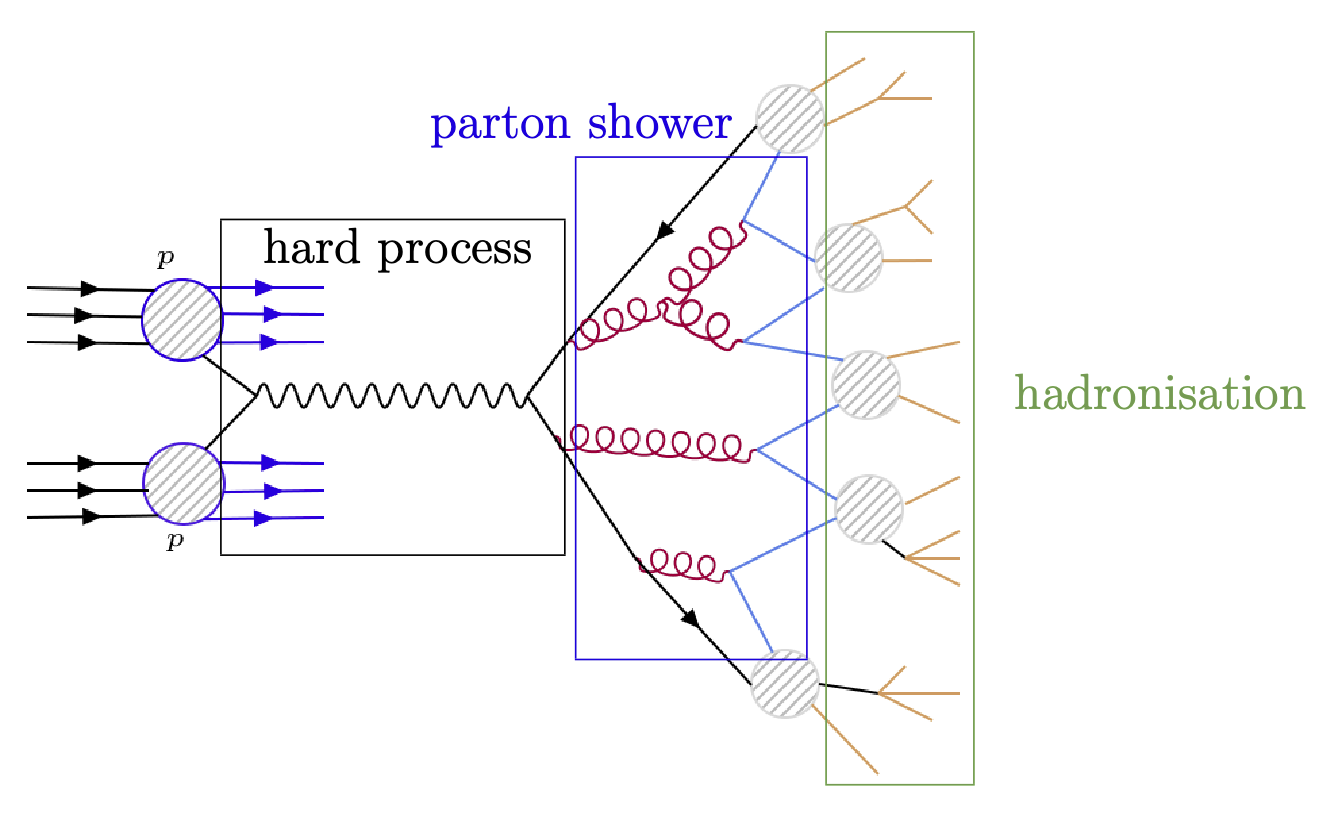
\includegraphics[width=0.8\textwidth]{plots/chapter4/simulation.png}
  \caption{MC simulation of an event in \pp collisions.}
  \label{fig:simulation}
\end{figure}


\section{Monte Carlo simulation}

The primary hard interaction process and the decay of short-lived particles happen at short distance scales. The QCD and QED radiation at a time scale much below $\frac{1}{\Lambda}$, where $\Lambda$ is a typical hadronic scale of a few hundred~\MeV, are also happening at short distance scales. Soft and collinear safe inclusive observables, such as total decay widths or inclusive cross-sections, can be computed with pQCD theory for momentum scales much larger than this scale. The final state collinear splittings and soft emissions give rise to large logarithmically divergent corrections, which cancel against virtual corrections in the total cross-section. Initial state collinear singularities are factorized into parton distribution functions (PDFs). Therefore, the cross-section remains accurate up to higher-order corrections if interpreted as an inclusive cross-section. If this is not the case, then the QCD singularities can lead to a non-convergence of the fixed order expansion.

\textbf{Matrix element generator:} Matrix element generators generate the exact matrix elements for the production of the process. They also produce a certain number of additional partons for hard, large-angle emissions. The radiation of extra partons is not included at the tree level accuracy of the hard process. The radiation of an extra parton with tree level accuracy can be included to provide next to leading order (NLO) corrections along with all NLO virtual corrections. The parton shower algorithms use as input the final state partons of the hard process and their phase space.

\textbf{Parton shower algorithm:} The parton shower algorithm is used for computing the cross-section for a generic hard process. Parton level events are transferred from a hard process generator to a shower generator, containing a list of particles and the used free parameters, using the Les Houches Event File standard~\cite{Alwall:2006yp}. The kinematics of the basic process is first generated, followed by a sequence of independent shower splittings. The cross-section for the given final state is calculated by assigning a probability to each splitting vertex. Collinear emissions and soft gluon emissions at arbitrary angles are the two sources of infrared singularities in massless field theories like QCD. PYTHIA uses a $\text{p}_{\perp}$ ordered shower evolution for correctly describing both effects.

\textbf{Matching:} QCD color confinement restricts quarks and gluons from existing as isolated particles. The hadronization of a quark or a gluon gives rise to hadrons or their decay products. Jets are collimated bunches of these hadrons. The collinear/soft radiation of an appropriate (N + 1) parton final state, generated by a matrix element generator, can give rise to a (N + 1) jet event. A (N + 1) jet event can also be obtained from an N parton final state with hard, large-angle emission during shower evolution. A matching has to be done if different generators have been used to generate matrix elements and parton showers or extra partons generated by the hard process generator.

\textbf{Hadronization models:} The hadronization scale $\text{Q}_{\text{had}}$ is by construction equal to the infrared cut-off where the parton shower ends. Colored partons are transformed into a set of colorless hadrons by GPMCs. This happens at scales with low momentum transfers and at long distances, where non-perturbative effects become important. GPMCs use models that rely on the color flow information between partons as a starting point for hadronization.

\textbf{Soft hadron-hadron physics modeling :} Underlying event is the additional activity beyond the basic process and its associated initial state and final state radiation. The dominant part is coming from additional color exchanges between the beam remnants. Multiple parton-parton interactions (MPI) can produce two or more back-to-back jet pairs, with each pair having a small transverse momentum. Most MPI are soft, and they influence the color flow and the event's total scattered energy. This increases the particle multiplicity in the final state and affects the final state activity. Compared to events with no hard jets, the hard jets appear to sit on top of a higher ``pedestal'' of underlying activity. This comes from the impact parameter dependence since central collisions are more likely to contain at least one hard scattering due to the higher probability of interactions and is called the ``jet pedestal'' effect.

\textbf{Parameter Tuning:} The accuracy of the used models is very important for event simulation. The accuracy depends on the inclusiveness of the chosen observables and the sophistication of the simulation. The models can be improved by improving the theoretical calculations. The precision also depends on the constraints in the free parameters, and existing collision data constrains them and is referred to as generator tuning. MC generators are not tuned beyond the constraints in theoretical and experimental precision to avoid overfitting. The final state of the particles and their spectra are influenced by event modeling and generator tuning. Events generated with different generators or tunes can differ and might not describe the collision data in the entire phase space.


\section{Monte Carlo generators}

PYTHIA has been developed for multi-particle production in \pp collisions and simulation of jets. PYTHIA can generate hard subprocess, initial and final state parton showers, hadronization, decays, and the underlying event. Many hard processes have been implemented for generating the matrix elements for final state and phase space calculation. PYTHIA can optimally generate $2 \to 1$ and $2 \to 2$ processes. Resonance decays with the resonance masses above the b quark system are implemented. Their branching fractions and partial width can be dynamically calculated as a function of their mass. If the spin information is available for resonance decays, it leads to angular correlations of the resonance decay products; otherwise, the resonance decays isotropically. GPMC generators like PYTHIA can simulate the full process. However, there are specialized generators that deal with a certain aspect of the event simulation.

\textbf{MadGraph:} MadGraph generates the matrix element with leading order (LO) accuracy~\cite{Alwall:2011uj}. MadGraph is a matrix element generator for processes that involve final states with a large number of jets, heavy flavor quarks, leptons, and missing energy. Events from new physics models that are renormalizable or from an effective field theory written in a Lagrangian can be generated. The full amplitude is split into gauge invariant sub-amplitudes. The matrix element contains the full spin correlation and Breit-Wigner effects but is not valid far from the mass peak.

\textbf{POWHEG:} POWHEG is a framework for implementing NLO matrix element calculations~\cite{Alioli:2010xd}. It includes NLO virtual corrections and radiation of an extra parton in the matrix element. It needs the LO matrix elements and the finite part of the virtual corrections as input from which it finds all the singular regions. The singular regions are characterized by a final state parton becoming collinear or soft to either an initial state parton or a final state parton. The singular regions can be grouped according to their underlying LO diagram by replacing this parton pair with a single parton of appropriate flavor.

\textbf{aMC@NLO:} aMC@NLO implements all aspects of NLO computation and its matching with parton showers~\cite{Frederix:2011ss, Alwall:2014hca}. NLO calculations can be achieved by combining one-loop matrix elements and tree-level matrix elements. Tree level computations are performed using MadGraph, and one-loop amplitudes are evaluated with MadLoop~\cite{Hirschi:2011pa}. The matched samples which differ by their final state multiplicity can be merged using the FxFx merging scheme.

\textbf{MLM matching:} MLM matching scheme is a matching algorithm~\cite{Mangano:2001xp, Mangano:2002ea} that matches partons from matrix element calculations to jets reconstructed after shower generation. Parton level events are required to have a separation greater than a minimum value $\text{R}_{\text{jj}} > \text{R}_{\text{min}}$ between them and at least a minimum transverse energy $\text{E}^{\text{min}}_{\text{T}}$ for partons. The jet closest in $(\eta, \phi)$ to the hardest parton is selected, and both match if the distance is smaller than $\text{R}_{\text{min}}$. Once a match is found, the jet is removed, and matching is done with the next parton. If a match is not found, then the event is rejected. This is the case for collinear partons or soft partons, which do not lead to an independent jet or are too soft for jet reconstruction.

\textbf{FxFx merging:} FxFx merging scheme is an NLO merging procedure~\cite{Frederix:2012ps}. There can be NLO accuracy for exclusive events with J light jets by the computation based on matrix elements that have J and (J + 1) partons. NLO mergings are more complicated than LO ones. This is because the matrix elements are considered twice, as Born contribution for processes with J partons and as the real emission contribution, infrared subtraction terms, and the one-loop contributions to processes with (J - 1) partons. Events are reweighted, and a certain amount of events might carry negative weights.


\section{Detector simulation}

In detector simulation, the interactions of particles with the detector material and the detector response are simulated. These events can then be reconstructed and analyzed. Geant4~\cite{Agostinelli:2002hh} is used for detector simulation. It is a toolkit for simulating particles' passage through matter and for simulating particle interactions with matter across a very wide energy range. The user defines the detector geometry and materials. A large number of components with different shapes and materials can be included in the geometrical model. Sensitive elements can be defined, which record information in the form of hits. Hits are needed to simulate the detector responses called digitization. The detector's geometrical structure is divided into logical and physical volumes. Logical volumes contain the information of the material and the sensitive detector behavior. A mixture of different elements and isotopes can be used for the material. Physical volumes carry information about the spatial positioning or placement of the logical volumes.

Particles can interact with the detector material or can decay while they are transported through the geometry. A model can be implemented by electromagnetic and hadronic processes in Geant4 depending on the energy or particle type. Geant4 can handle ionization described by energy loss and range tables, bremsstrahlung, pair production of electron-positrons from photons, photoelectric effect, pair conversion, annihilation, synchrotron, and transition radiation, scintillation, refraction, reflection, absorption, the Cherenkov effect, and many other processes. Particles with their basic properties, like mass, charge, and sensitive processes, can be defined. Particles are transported in steps, and they are tracked through materials and external electromagnetic fields. Event data is generated during simulation. First, events contain primary vertices and primary particles before processing an event. After processing, hits and digitizations generated by simulation are added. Trajectories of simulated particles can be added optionally for the recording of ``simulation truth.''


\section{Monte Carlo samples}

MC simulated event samples are used to model signal and background contributions to all the analysis regions with several event generators. In all cases, parton showering, hadronization, and underlying event properties are modeled using PYTHIA version 8.212. The PYTHIA parameters affecting the description of the underlying event are set to the CUETP8M1 tune in 2016~\cite{Khachatryan:2015pea}, except for the \ttbar sample where the CP5 tune is used, which is also the tune in 2017 and 2018~\cite{CMS:2018zub}. The NNPDF3.0 PDF set is used for all 2016 samples, and the NNPDF3.1 PDF set is used for the 2017 and 2018 samples~\cite{Ball:2017nwa}.

Simulation of interactions between particles and the CMS detector is based on Geant4. The same reconstruction algorithms used for data are applied to simulated samples as well. The Higgs bosons are produced in \pp collisions predominantly by gluon gluon fusion (ggF)~\cite{Georgi:1977gs}, but also by vector boson fusion (VBF)~\cite{Cahn:1986zv}, and in association with a vector boson (W/Z)~\cite{Glashow:1978ab}. The ggF, VBF, and associated production Higgs boson samples are generated with POWHEG generator in the implementation described in Ref.~\cite{Heinrich:2017kxx, Buchalla:2018yce}. We only consider Higgs boson produced in ggF and VBF production mechanisms and do not use associated production Higgs boson samples for the signal.

Embedded samples are data samples with well-identified \Zmm events from which muons are removed, and simulated tau leptons are embedded with the same kinematics as the replaced muons. These samples are employed for the data-driven estimation of the \Ztt and some \ttbar/Diboson/Single Top background. The MadGraph generator is used to simulate the $\Zee/\Pgm{}\Pgm + \text{jets}$ process along with the \wjets background process. They are simulated at LO with MLM jet matching and merging schemes~\cite{Alwall:2007fs}.

Diboson production is simulated at NLO using aMC@NLO generator with FxFx jet matching and merging scheme. Top quark pair and single top quark production simulated samples are generated using POWHEG. Due to the high instantaneous luminosities attained during data taking, events have multiple \pp interactions per bunch crossing. The effect is taken into account in simulated samples by generating concurrent minimum bias events. All simulated samples are weighted to match the pileup distribution observed in the data.
